% Options for packages loaded elsewhere
\PassOptionsToPackage{unicode}{hyperref}
\PassOptionsToPackage{hyphens}{url}
%
\documentclass[
]{article}
\usepackage{amsmath,amssymb}
\usepackage{lmodern}
\usepackage{setspace}
\usepackage{iftex}
\ifPDFTeX
  \usepackage[T1]{fontenc}
  \usepackage[utf8]{inputenc}
  \usepackage{textcomp} % provide euro and other symbols
\else % if luatex or xetex
  \usepackage{unicode-math}
  \defaultfontfeatures{Scale=MatchLowercase}
  \defaultfontfeatures[\rmfamily]{Ligatures=TeX,Scale=1}
\fi
% Use upquote if available, for straight quotes in verbatim environments
\IfFileExists{upquote.sty}{\usepackage{upquote}}{}
\IfFileExists{microtype.sty}{% use microtype if available
  \usepackage[]{microtype}
  \UseMicrotypeSet[protrusion]{basicmath} % disable protrusion for tt fonts
}{}
\makeatletter
\@ifundefined{KOMAClassName}{% if non-KOMA class
  \IfFileExists{parskip.sty}{%
    \usepackage{parskip}
  }{% else
    \setlength{\parindent}{0pt}
    \setlength{\parskip}{6pt plus 2pt minus 1pt}}
}{% if KOMA class
  \KOMAoptions{parskip=half}}
\makeatother
\usepackage{xcolor}
\usepackage[margin=1in]{geometry}
\usepackage{longtable,booktabs,array}
\usepackage{calc} % for calculating minipage widths
% Correct order of tables after \paragraph or \subparagraph
\usepackage{etoolbox}
\makeatletter
\patchcmd\longtable{\par}{\if@noskipsec\mbox{}\fi\par}{}{}
\makeatother
% Allow footnotes in longtable head/foot
\IfFileExists{footnotehyper.sty}{\usepackage{footnotehyper}}{\usepackage{footnote}}
\makesavenoteenv{longtable}
\usepackage{graphicx}
\makeatletter
\def\maxwidth{\ifdim\Gin@nat@width>\linewidth\linewidth\else\Gin@nat@width\fi}
\def\maxheight{\ifdim\Gin@nat@height>\textheight\textheight\else\Gin@nat@height\fi}
\makeatother
% Scale images if necessary, so that they will not overflow the page
% margins by default, and it is still possible to overwrite the defaults
% using explicit options in \includegraphics[width, height, ...]{}
\setkeys{Gin}{width=\maxwidth,height=\maxheight,keepaspectratio}
% Set default figure placement to htbp
\makeatletter
\def\fps@figure{htbp}
\makeatother
\setlength{\emergencystretch}{3em} % prevent overfull lines
\providecommand{\tightlist}{%
  \setlength{\itemsep}{0pt}\setlength{\parskip}{0pt}}
\setcounter{secnumdepth}{5}
\usepackage{lineno}
\linenumbers
\newcommand{\beginsupplement}{\setcounter{table}{0}  \renewcommand{\thetable}{S\arabic{table}} \setcounter{figure}{0} \renewcommand{\thefigure}{S\arabic{figure}}}
\usepackage{float}
\usepackage{booktabs}
\usepackage{caption}
\usepackage{longtable}
\ifLuaTeX
  \usepackage{selnolig}  % disable illegal ligatures
\fi
\IfFileExists{bookmark.sty}{\usepackage{bookmark}}{\usepackage{hyperref}}
\IfFileExists{xurl.sty}{\usepackage{xurl}}{} % add URL line breaks if available
\urlstyle{same} % disable monospaced font for URLs
\hypersetup{
  pdftitle={IMF and Benchmark Forecasts},
  hidelinks,
  pdfcreator={LaTeX via pandoc}}

\title{IMF and Benchmark Forecasts}
\author{}
\date{\vspace{-2.5em}}

\begin{document}
\maketitle

\setstretch{2}
\hypertarget{a-short-note-on-error-handling}{%
\section{A short note on error handling}\label{a-short-note-on-error-handling}}

In almost all 72 cases, absolute error handling gives lower scores than directional error handling. The only exception is the inflation series for the IMF forecasts and horizon 0, where the expanding window and rolling window method give \textit{slightly} lower scores for the directional methodology.
We thus decide to focus on the absolute errors in this document.

\hypertarget{scores-by-estimation-method-horizon-and-forecast-source}{%
\section{Scores, by estimation method, Horizon and forecast source}\label{scores-by-estimation-method-horizon-and-forecast-source}}

\begin{longtable}{l|rrr}
\toprule
\multicolumn{1}{l}{} & IMF & ar & bvar \\ 
\midrule
\multicolumn{4}{l}{horizon = 0} \\ 
\midrule
expanding window\_interval\_score & 0.115 & 0.123 & 0.122 \\ 
expanding window\_sample\_crps & 0.087 & 0.092 & 0.091 \\ 
leave-one-out\_interval\_score & 0.119 & 0.133 & 0.134 \\ 
leave-one-out\_sample\_crps & 0.088 & 0.099 & 0.100 \\ 
rolling window\_interval\_score & 0.119 & 0.128 & 0.126 \\ 
rolling window\_sample\_crps & 0.094 & 0.097 & 0.098 \\ 
\midrule
\multicolumn{4}{l}{horizon = 0.5} \\ 
\midrule
expanding window\_interval\_score & 0.258 & 0.272 & 0.296 \\ 
expanding window\_sample\_crps & 0.182 & 0.208 & 0.241 \\ 
leave-one-out\_interval\_score & 0.261 & 0.313 & 0.317 \\ 
leave-one-out\_sample\_crps & 0.180 & 0.217 & 0.230 \\ 
rolling window\_interval\_score & 0.261 & 0.266 & 0.288 \\ 
rolling window\_sample\_crps & 0.191 & 0.201 & 0.235 \\ 
\midrule
\multicolumn{4}{l}{horizon = 1} \\ 
\midrule
expanding window\_interval\_score & 0.448 & 0.737 & 0.590 \\ 
expanding window\_sample\_crps & 0.327 & 0.504 & 0.426 \\ 
leave-one-out\_interval\_score & 0.427 & 0.726 & 0.600 \\ 
leave-one-out\_sample\_crps & 0.302 & 0.448 & 0.400 \\ 
rolling window\_interval\_score & 0.451 & 0.739 & 0.591 \\ 
rolling window\_sample\_crps & 0.333 & 0.514 & 0.434 \\ 
\midrule
\multicolumn{4}{l}{horizon = 1.5} \\ 
\midrule
expanding window\_interval\_score & 0.495 & 1.044 & 0.800 \\ 
expanding window\_sample\_crps & 0.346 & 0.627 & 0.602 \\ 
leave-one-out\_interval\_score & 0.487 & 1.103 & 0.903 \\ 
leave-one-out\_sample\_crps & 0.337 & 0.583 & 0.577 \\ 
rolling window\_interval\_score & 0.494 & 1.041 & 0.779 \\ 
rolling window\_sample\_crps & 0.347 & 0.632 & 0.570 \\ 
\bottomrule
\end{longtable}

\hypertarget{inflation}{%
\subsection{Inflation}\label{inflation}}

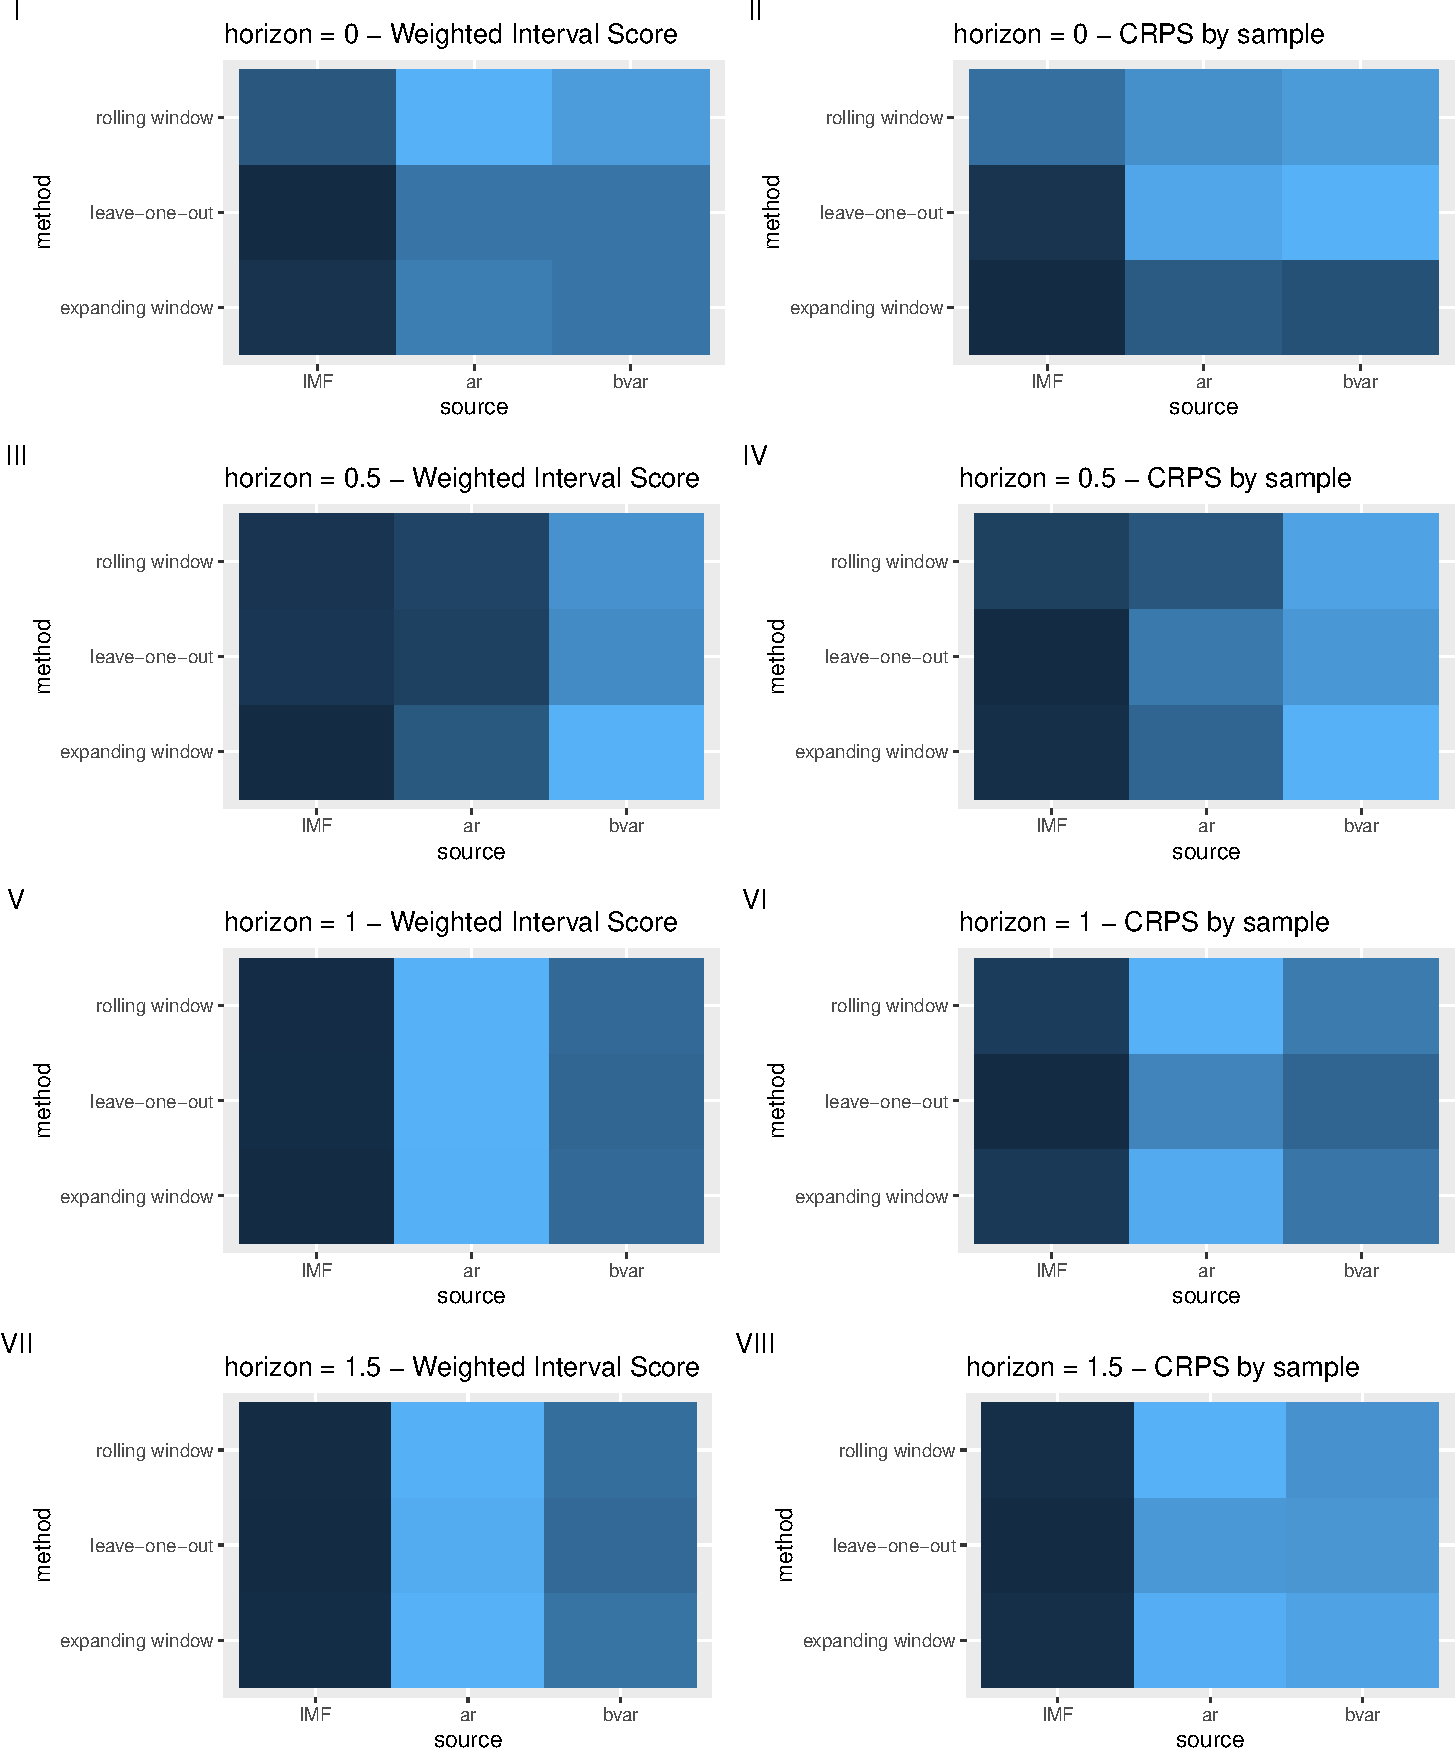
\includegraphics{manuscript_files/figure-latex/unnamed-chunk-2-1.pdf}

\hypertarget{gdp}{%
\subsection{GDP}\label{gdp}}

\begin{longtable}{l|rrr}
\toprule
\multicolumn{1}{l}{} & IMF & ar & bvar \\ 
\midrule
\multicolumn{4}{l}{horizon = 0} \\ 
\midrule
expanding window\_interval\_score & 0.241 & 0.301 & 0.298 \\ 
expanding window\_sample\_crps & 0.178 & 0.209 & 0.204 \\ 
leave-one-out\_interval\_score & 0.257 & 0.312 & 0.310 \\ 
leave-one-out\_sample\_crps & 0.183 & 0.219 & 0.214 \\ 
rolling window\_interval\_score & 0.240 & 0.302 & 0.297 \\ 
rolling window\_sample\_crps & 0.178 & 0.211 & 0.204 \\ 
\midrule
\multicolumn{4}{l}{horizon = 0.5} \\ 
\midrule
expanding window\_interval\_score & 0.416 & 0.540 & 0.493 \\ 
expanding window\_sample\_crps & 0.298 & 0.383 & 0.358 \\ 
leave-one-out\_interval\_score & 0.448 & 0.583 & 0.531 \\ 
leave-one-out\_sample\_crps & 0.310 & 0.408 & 0.377 \\ 
rolling window\_interval\_score & 0.416 & 0.554 & 0.504 \\ 
rolling window\_sample\_crps & 0.297 & 0.405 & 0.373 \\ 
\midrule
\multicolumn{4}{l}{horizon = 1} \\ 
\midrule
expanding window\_interval\_score & 0.837 & 1.090 & 0.942 \\ 
expanding window\_sample\_crps & 0.640 & 0.822 & 0.763 \\ 
leave-one-out\_interval\_score & 0.858 & 1.067 & 0.948 \\ 
leave-one-out\_sample\_crps & 0.634 & 0.759 & 0.709 \\ 
rolling window\_interval\_score & 0.851 & 1.122 & 0.970 \\ 
rolling window\_sample\_crps & 0.663 & 0.875 & 0.815 \\ 
\midrule
\multicolumn{4}{l}{horizon = 1.5} \\ 
\midrule
expanding window\_interval\_score & 1.045 & 1.288 & 1.102 \\ 
expanding window\_sample\_crps & 0.790 & 0.937 & 0.897 \\ 
leave-one-out\_interval\_score & 1.034 & 1.278 & 1.107 \\ 
leave-one-out\_sample\_crps & 0.765 & 0.882 & 0.849 \\ 
rolling window\_interval\_score & 1.056 & 1.312 & 1.143 \\ 
rolling window\_sample\_crps & 0.831 & 0.985 & 0.949 \\ 
\bottomrule
\end{longtable}

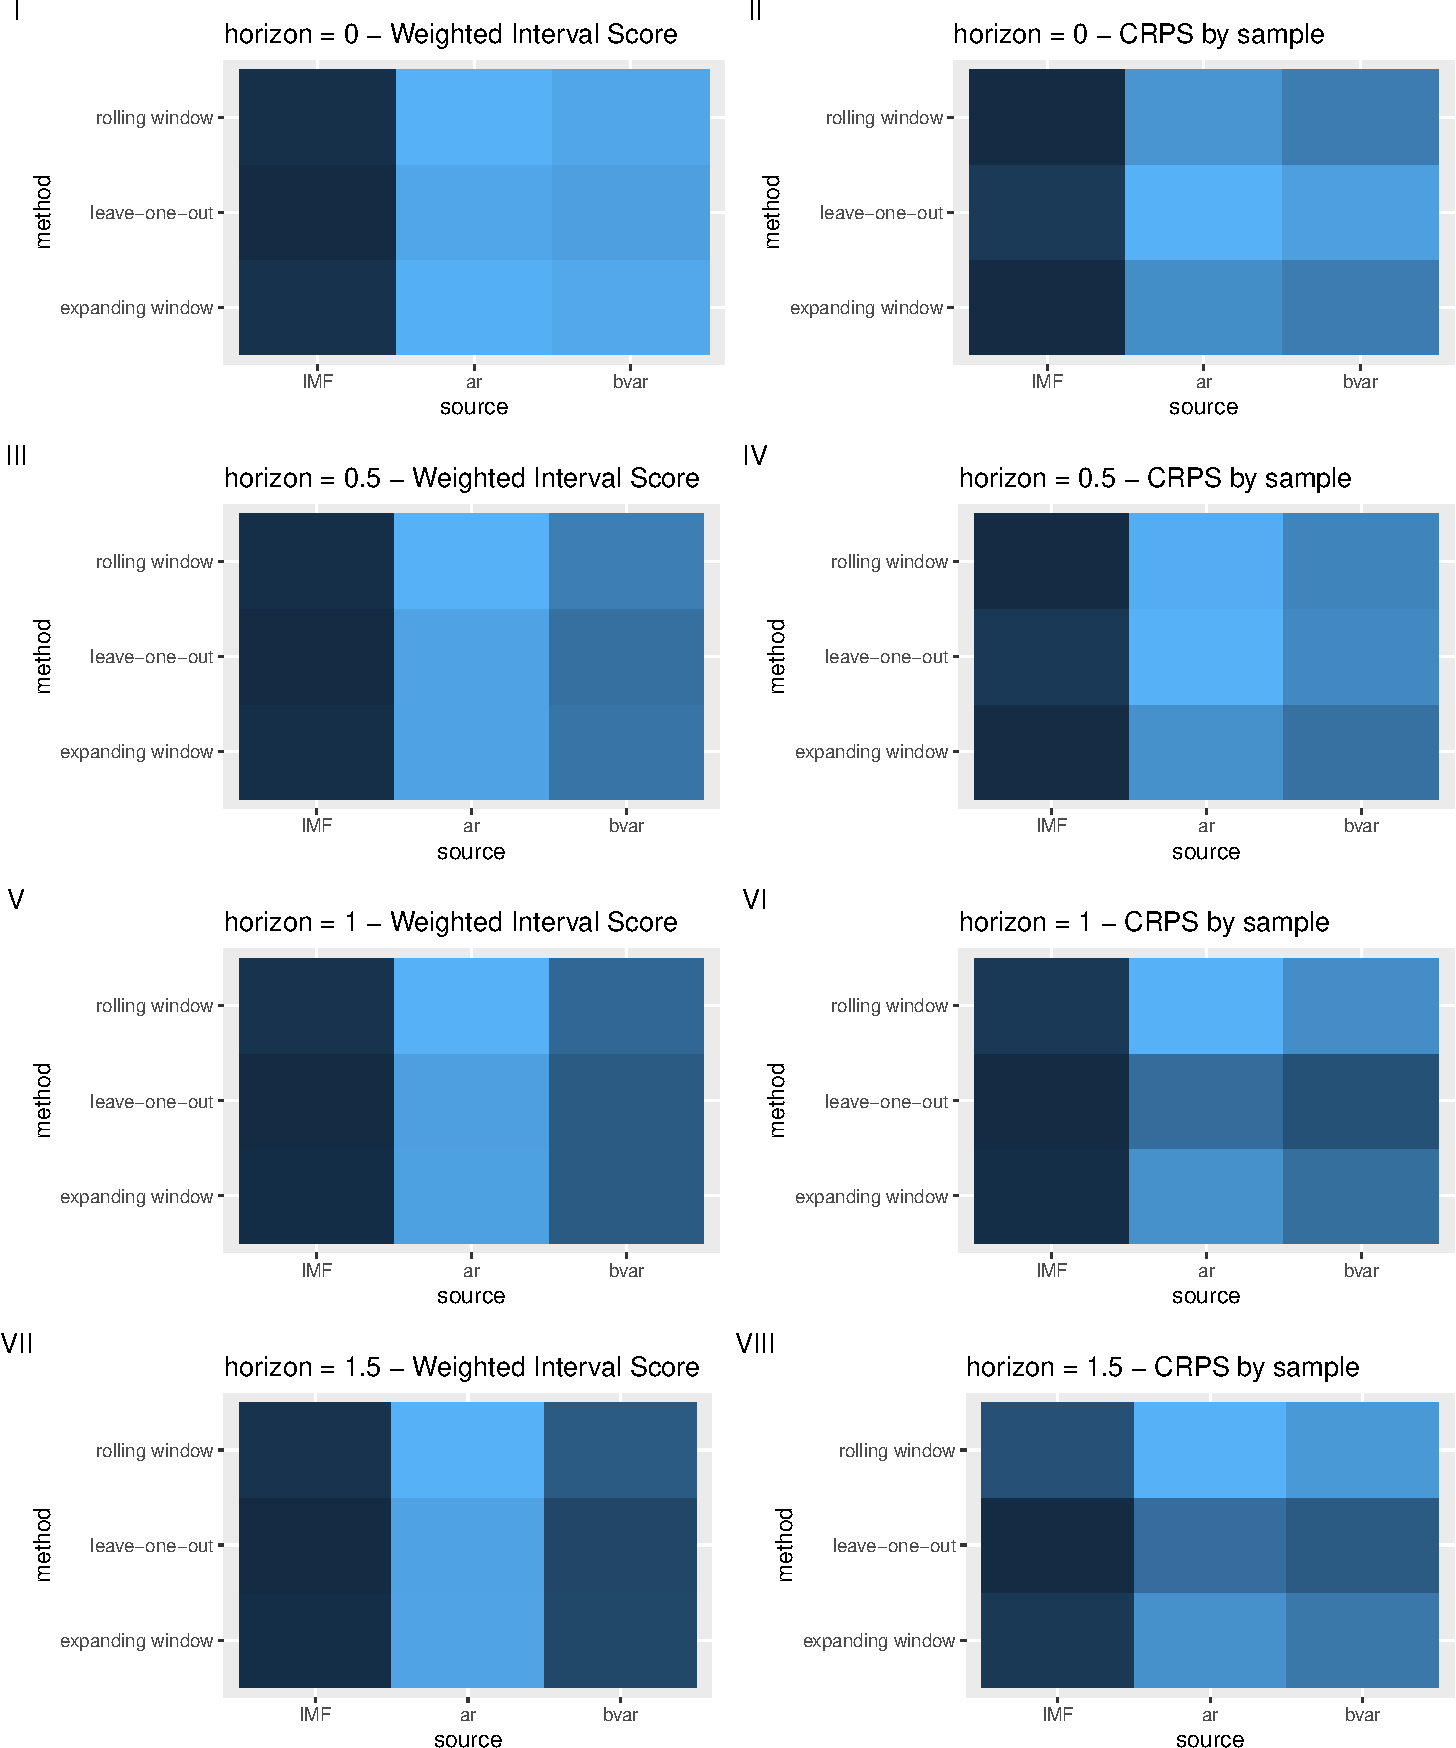
\includegraphics{manuscript_files/figure-latex/unnamed-chunk-3-1.pdf}

\hypertarget{coverage-by-target-methods-and-source}{%
\section{Coverage, by target, methods and source}\label{coverage-by-target-methods-and-source}}

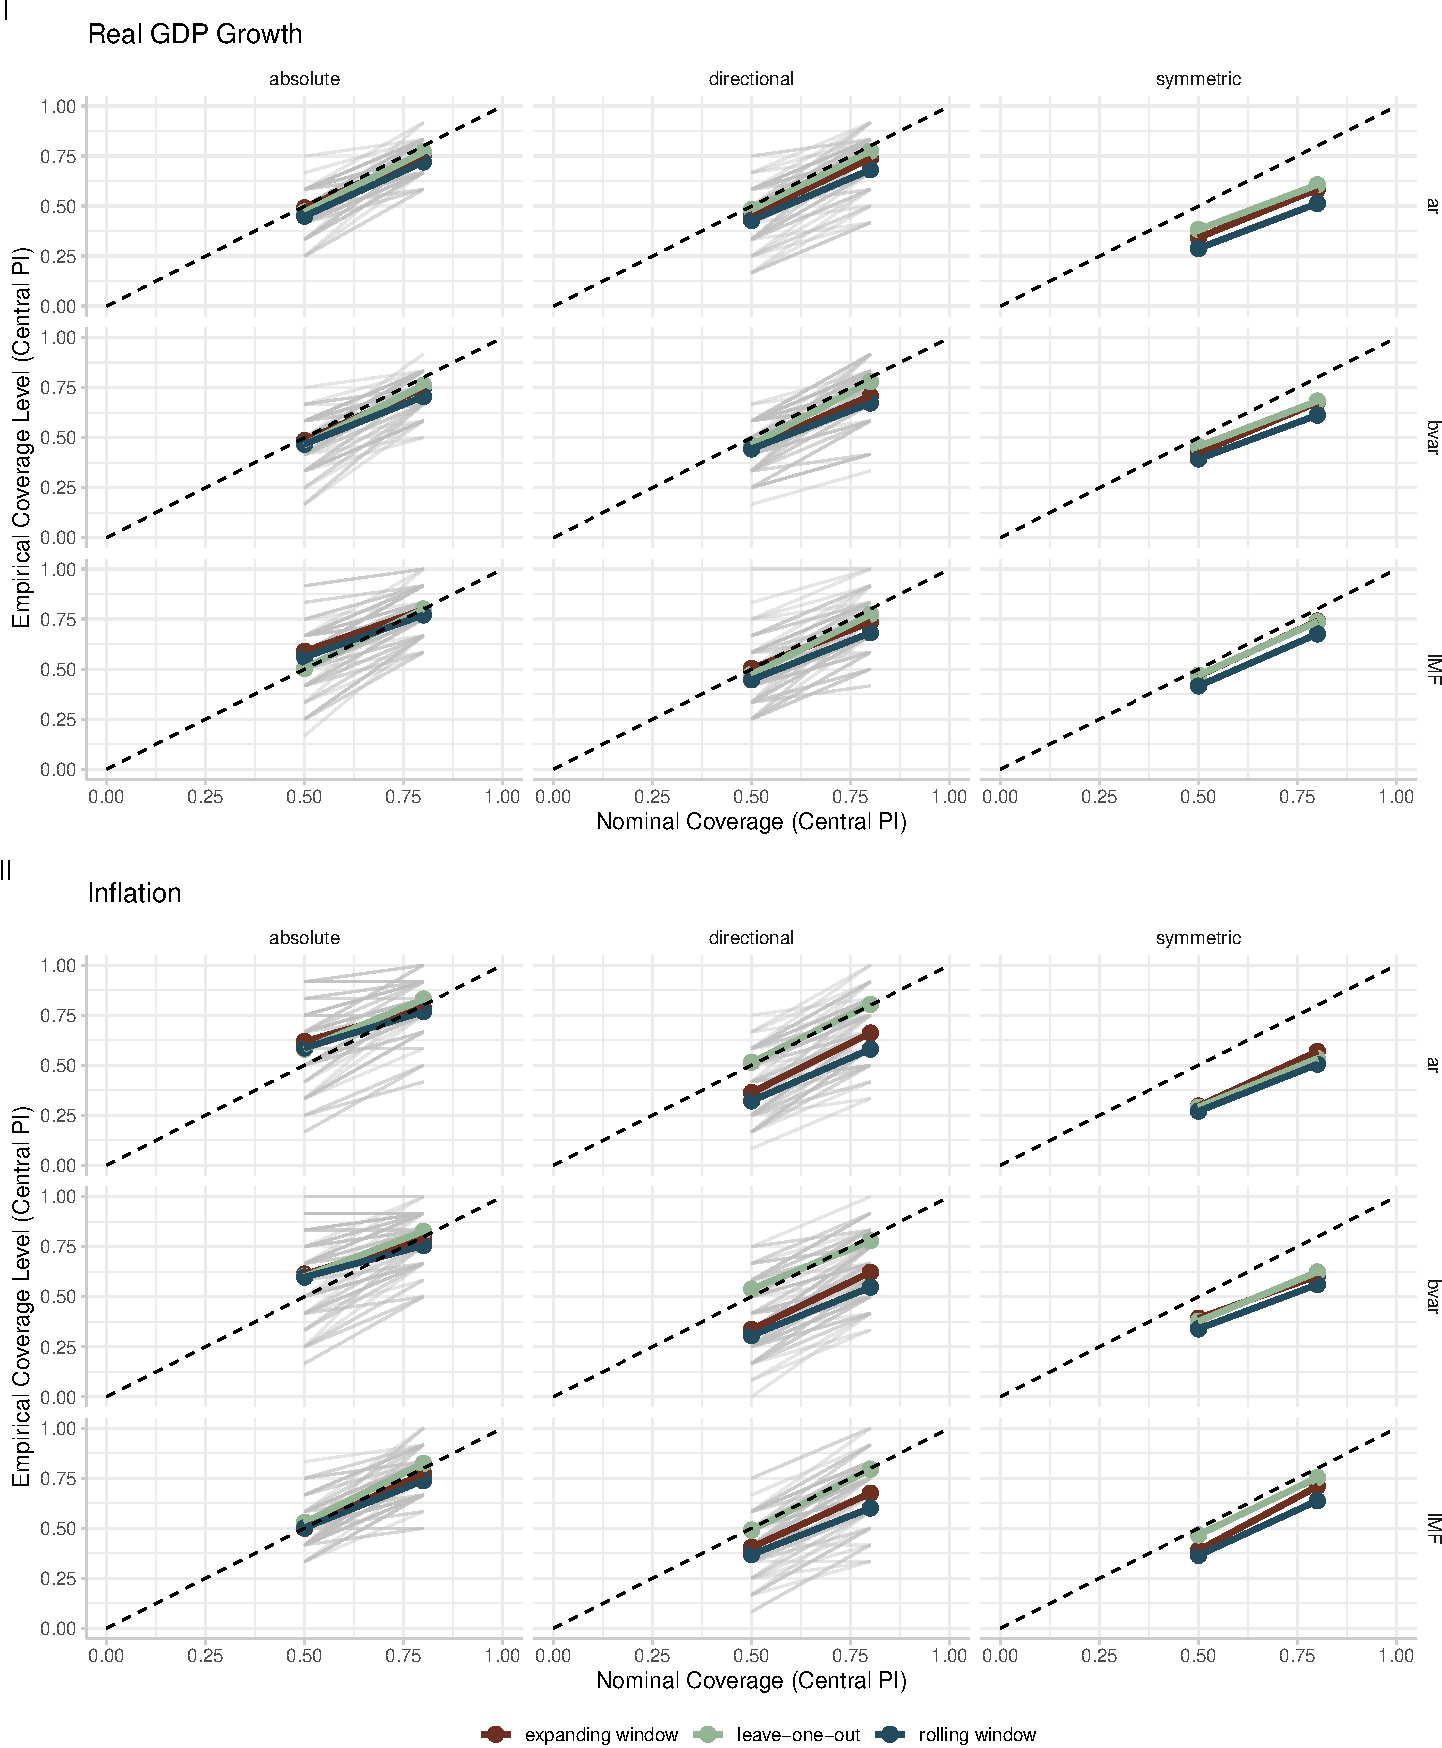
\includegraphics{manuscript_files/figure-latex/cvgplot-1.pdf}

\end{document}
